
This day will serve as an introduction to machine learning. We recall some fundamental concepts 
about decision theory and classification. We also present some widely used models and algorithms 
and try to provide the main motivation behind them. 
There are several textbooks that provide a thorough description of some of the concepts introduced here: 
for example, \citet{Mitchell1997},\citet{Duda2001}, \citet{Schoelkopf2002}, \citet{Joachims2002}, \citet{Bishop2006}, \citet{Manning2008}, 
to name just a few.  
The concepts that we introduce in this chapter will be revisited in later chapters, where the same algorithms and models 
will be adapted to structured inputs and outputs. For now, we concern only with multi-class classification 
(with just a few classes). 

\section*{Today's assignment}

The assignment of today's class is to implement a classifier called Naive Bayes, and use it to perform sentiment analysis on a corpus of book reviews from Amazon.

\section{Pre-assignment}

\subsection{Notation}

In what follows, we denote by $\mathcal{X}$ our \emph{input set} (also called \emph{observation set}), and by $\mathcal{Y}$ our \emph{output set}. 
We will make no assumptions about the set $\mathcal{X}$, which can be continuous or discrete. In this lecture, we 
consider \emph{classification} problems, where $\mathcal{Y} = \{c_1,\ldots,c_K\}$ is a finite set, consisting of $K$ \emph{classes} (also called \emph{labels}). 
For example, $\mathcal{X}$ can be a set of documents in natural language, and $\mathcal{Y}$ a set of topics, the goal 
being to assign a topic to each document. 

We use upper-case letters for denoting random variables, and lower-case letters for value assignments to those variables:  
for example, 
\begin{itemize}
\item $X$ is a random variable taking values on $\mathcal{X}$,
\item $Y$ is a random variable taking values on $\mathcal{Y}$,
\item $x \in \mathcal{X}$ and $y \in \mathcal{Y}$ are particular values for $X$ and $Y$. 
\end{itemize}  
We consider \emph{events} such as $X=x$, $Y=y$, etc. 
Throughout, we use modified notation and let $P(y)$ denote the \emph{probability} associated with the event $Y=y$ (instead of writing $P_Y(Y=y)$). 
\emph{Joint} and \emph{conditional} probabilities are 
denoted respectively as $P(x,y) \triangleq P_{X,Y}(X=x \wedge Y=y)$ and $P(x|y) \triangleq P_{X|Y}(X=x \,\,|\,\,Y=y)$. From the laws of probabilities: 
\begin{equation}
P(x,y)=P(y|x) P(x) = P(x|y) P(y), 
\end{equation}
for all $x \in \mathcal{X}$ and $y \in \mathcal{Y}$.

Quantities that are predicted or estimated from the data will be appended a hat-symbol: for example, estimations of the probabilities above are denoted 
as ${\hat P}(y)$, ${\hat P}(x,y)$ and ${\hat P}(y|x)$; and a prediction of an output will be denoted ${\hat y}$. 

We assume that a \emph{training dataset} $\mathcal{D}$ is provided
which consists of $M$ input-output pairs (called \emph{examples} or
\emph{instances}): 
\begin{equation}
\mathcal{D} = \{(x^{1},y^{1}),\ldots,(x^{M},y^{M})\} \subseteq \mathcal{X} \times \mathcal{Y}.  
\end{equation}

The goal of (supervised) machine learning is to use the training dataset $\mathcal{D}$ to learn a function $h$ (called a \emph{classifier}) 
that maps from $\mathcal{X}$ to $\mathcal{Y}$: this way, given a new instance 
$x \in \mathcal{X}$ (test example), the machine makes a prediction ${\hat y}$ by evaluating $h$ on $x$, i.e., ${\hat y} = h(x)$. 

%\out{
\begin{figure}
\begin{center}
    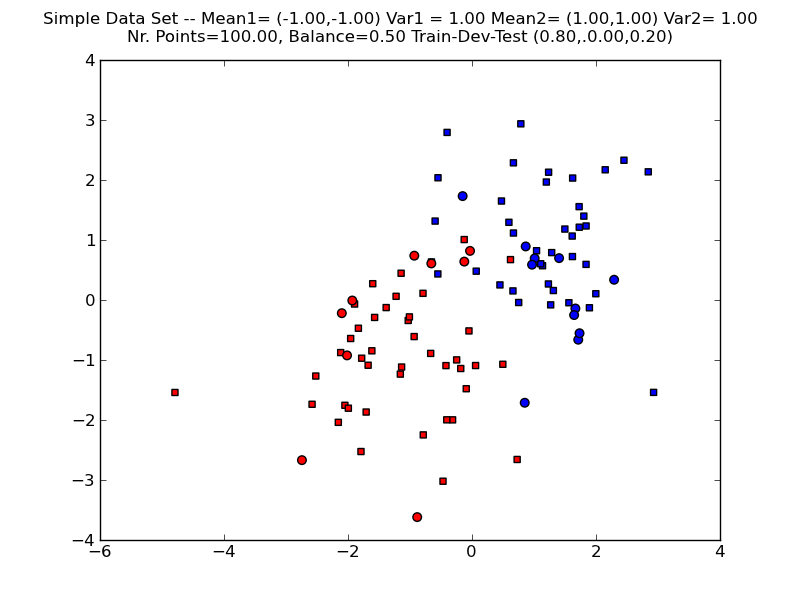
\includegraphics[width=1\columnwidth]{figs/classification/simple_data_set}
  \caption{\label{simpleDataSet} Example of a dataset.
    The input set consists in points in the real plane, $\mathcal{X} =
    \mathbb{R}^2$, and the output set consists of two classes (Red
    and Blue). Training points are represented as squares, while test
    points are represented as circles.}
  \end{center}
\end{figure}
%}

\subsection{\label{s::naiveBayes}Generative Classifiers: Na\"{i}ve Bayes}

If we knew the \emph{true} distribution $P(X,Y)$, the best possible classifier (Bayes optimal) 
would be one which predicts according to

\begin{eqnarray}
{\hat y} &=& \arg\max_{y \in \mathcal{Y}} P(y|x) = \arg\max_{y \in \mathcal{Y}} \frac{P(x,y)}{P(x)} \nonumber\\
&=^{\dagger}& \arg\max_{y \in \mathcal{Y}} P(x,y) \nonumber \\
&=& \arg\max_{y \in \mathcal{Y}} P(y) P(x|y),
\end{eqnarray}
where in ${\dagger}$ we used the fact that $P(x)$ is constant with respect to $y$. Generative classifiers try to estimate the probability distributions $P(Y)$ and $P(X|Y)$ (which are respectively called the \emph{class prior} and the \emph{class conditionals}).
  
Figure \ref{simpleDataSet_bo} shows an example of
the Bayes optimal decision boundary for a toy example with $K=2$ classes, $M=100$ points, class priors $P(y_1) = P(y_2) = 0.5$, and class conditionals $P(x|y_i)$ given by 2-D Gaussian distributions with the same variance but different means.

\begin{figure}[h]
\begin{center}
    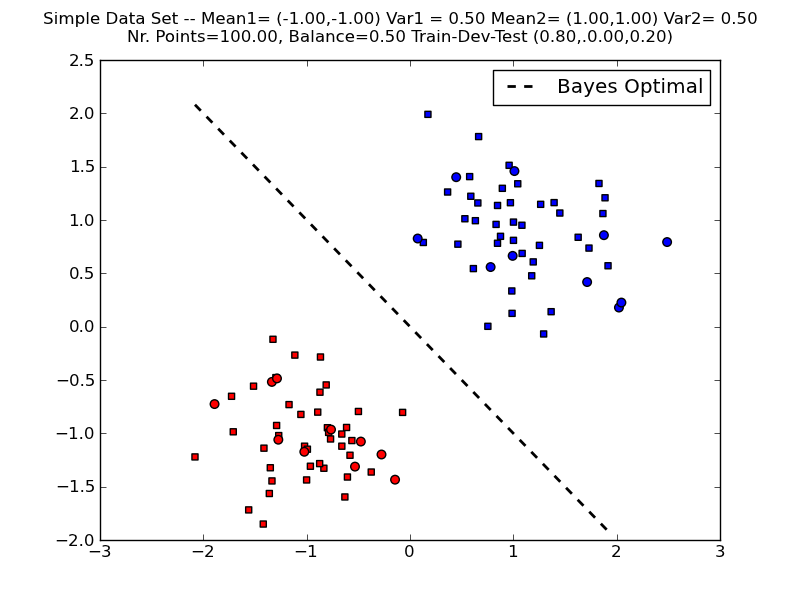
\includegraphics[width=1\columnwidth]{figs/classification/gaussian_separabale_bo.png}
  \caption{\label{simpleDataSet_bo} Example of a dataset together with
    the corresponding Bayes optimal decision boundary.
    The input set consists in points in the real plane, $\mathcal{X} =
    \mathcal{R^2}$, and the output set consists of two classes (Red
    and Blue). Training points are represented as squares, while test
    points are represented as circles.}
  \end{center}
\end{figure}



Generative models assume that the data are generated according to the following generative story (independently for each $m=1,\ldots,M$): 
\begin{enumerate}
\item A class $y_m \sim P(Y)$ is drawn from the class prior distribution;
\item An input $x_m \sim P(X|Y=y_m)$ is drawn from the corresponding class conditional.
\end{enumerate}
Training a generative model 
amounts to \emph{estimating} these probabilities using the dataset $\mathcal{D}$, yielding estimates 
$\hat{P}(y)$ and $\hat{P}(x|y)$. This estimation is usually called \emph{training}, or \emph{learning}.

After we are done training, we are given a new input $x \in \mathcal{X}$, and we want to make a prediction according to  
\begin{eqnarray}
{\hat y} &=& \arg\max_{y \in \mathcal{Y}} \hat{P}(y) \hat{P}(x|y),
\label{eq:argmax}
\end{eqnarray}
using the probabilities estimated in the training stage. This is usually called \emph{inference} or \emph{decoding}.


We are left with two important problems:
\begin{enumerate}
\item How should the distributions ${\hat P}(Y)$ and ${\hat P}(X|Y)$ be ``defined''?
(i.e., what kind of independence assumptions should they state, or how should they factor?)
\item How should parameters be estimated from the training data $\mathcal{D}$?
\end{enumerate}

The first problem strongly depends on the application at hand. Quite often, there is a natural decomposition of the input variable $X$ into $J$ components, 
\begin{equation}
X = (X_1,\ldots,X_J). 
\end{equation}
The na\"{i}ve Bayes method makes the following assumption: \emph{$X_1,\ldots,X_J$ are conditionally independent given the class}. Mathematically, this means that 
\begin{eqnarray}
P(X|Y) &=& \prod_{j=1}^J P(X_j|Y).
\end{eqnarray}
Note that this independence assumption greatly reduces the number of parameters to be estimated (degrees of freedom) 
from $O(\exp(J))$ to $O(J)$, 
hence estimation of ${\hat P}(X|Y)$ becomes much simpler, as we shall see. 
It also makes the overall computation much more efficient for large $J$ and it decreases the risk of overfitting the data. 
On the other hand, if the assumption is over-simplistic it may increase the risk 
of under-fitting. 
%This choice greatly simplifies the problem of parametrizing ${\hat P}(Y)$ and ${\hat P}(X|Y)$. 

For the second problem, one of the simplest ways to solve it is using \emph{maximum likelihood estimation}, which aims to maximize the probability of the training sample, assuming that each point was generated independently. This probability (call it $P(\mathcal{D})$) factorizes as 
\begin{eqnarray}
P(\mathcal{D}) &=& \prod_{m=1}^M P(x^m,y^m) \nonumber\\
&=& \prod_{m=1}^M P(y^m)\prod_{j=1}^J P(x^m_j|y^m). 
\end{eqnarray}



%%\begin{example}[2-D Gaussians] 
%\subsection{Example: 2-D Gaussians}
%
%We first illustrate the na\"ive Bayes assumption with a toy example. 
%Suppose that $\mathcal{X}=\mathbb{R}^2$ and $\mathcal{Y}=\{1,2\}$. 
%Assume that each class-conditional is a two-dimensional Gaussian distribution with fixed covariance, 
%i.e., $P(X_1,X_2|Y=y)=\mathcal{N}(\boldsymbol{\mu}_y, \boldsymbol{\Sigma}_y)$. 
%
%According to the na\"ive Bayes assumption, ${\hat P}(X_1,X_2|Y) = {\hat P}(X_1|Y) {\hat P}(X_2|Y)$ (remark: this 
%is equivalent to assuming that 
%the $\boldsymbol{\Sigma}_y$ are diagonal!). For simplicity, we also assume that the two classes have unit variance. Then, we have 
%${\hat P}(X_1|Y=y) = \mathcal{N}(\mu_{y1}, 1.0)$ 
%and ${\hat P}(X_2|Y=y) = \mathcal{N}(\mu_{y2}, 1.0)$. Figure
%\ref{simpleDataSet} shows an example a dataset of two gaussians with unit
%variance, where $\mu_{y1} = [-1,-1]$ and $\mu_{y1} = [1,1]$. Figure
%\ref{simpleDataSet_bo} shows the same example but where both
%gaussians have $\Sigma = 0.5$, together with the Bayes optimal decision boundary. 
%The parameters that need to be estimated are the class-conditional means $\mu_{11},\mu_{12},\mu_{21},\mu_{22}$ and 
%the class priors ${\hat P}(Y=1)$ and ${\hat P}(Y=2)$. Given a training sample $\mathcal{D} = \{(x^{1},y^{1}),\ldots,(x^{M},y^{M})\}$, 
%denote by $\mathcal{I}_1\subseteq \{1,\ldots,M\}$ the indices of those instances belonging to class $1$, and 
%by $\mathcal{I}_2\subseteq \{1,\ldots,M\}$ the indices of the ones that belong to class $2$. 
%The maximum likelihood estimates of the quantities above are: 
%\begin{eqnarray}
%{\hat P}(Y = 1) = \frac{|\mathcal{I}_1|}{M}, \quad 
%{\hat P}(Y = 2) = \frac{|\mathcal{I}_2|}{M}\nonumber\\
%\mu_{11} = \frac{1}{|\mathcal{I}_1|} \sum_{m \in \mathcal{I}_1} x_1^{m}, \quad
%\mu_{12} = \frac{1}{|\mathcal{I}_1|} \sum_{m \in \mathcal{I}_1} x_2^{m}\nonumber\\
%\mu_{21} = \frac{1}{|\mathcal{I}_2|} \sum_{m \in \mathcal{I}_2} x_1^{m}, \quad
%\mu_{22} = \frac{1}{|\mathcal{I}_2|} \sum_{m \in \mathcal{I}_2} x_2^{m}.
%\end{eqnarray}
%In words: the class priors' estimates are their relative frequencies, and 
%the class-conditional means' estimates are the sample means. 
%%\end{example}
%
%\begin{exercise}\label{exer:simplenb}
%
%\begin{enumerate}
%Start by importing all the libraries necessary for this lab through the following preamble: 
%\begin{python}
%import sys
%import matplotlib.pyplot as plt
%sys.path.append("readers/")
%sys.path.append("classifiers/")
%sys.path.append("distributions/")
%sys.path.append("util/")
%
%import simple_data_set as sds
%import linear_classifier as lcc
%import gaussian_naive_bayes as gnbc
%import naive_bayes as nb
%\end{python}
%
%Now, generate a training and a test dataset like in the previous example, each with $M=100$ points, $50$ of each class. 
%Assume the following class-conditionals: 
%$P(X|Y=1) \sim N((-1,-1), \sigma^2 \boldsymbol{I})$ and $P(X|Y=2) \sim
%N((1,1), \boldsymbol{I})$, for $\sigma = 1.0$. 
%To do this, run the following command from the {\tt code} directory:
%
%\begin{python}
%sd = sds.SimpleDataSet(nr_examples=100, g1 = [[-1,-1],1], g2 = [[1,1],1], balance=0.5, split=[0.5, 0, 0.5])
%\end{python}
%
%You can visualize your data and see the Bayes optimal surface boundary by typing: 
%\begin{python}
%fig,axis = sd.plot_data()
%\end{python}
%
%Note: you might need to type {\tt plt.show()} in order to show the figure.
%
%Now, run na\"ive Bayes on this dataset. To do that, use the class {\tt GaussianNaiveBayes}, 
%which is defined in the file {\tt GaussianNaiveBayes.py} under the
%classification directory. 
%Report your estimates, as well as training set and testing set
%accuracies:
%
%\begin{python}
%gnb = gnbc.GaussianNaiveBayes()
%params_nb_sd = gnb.train(sd.train_X, sd.train_y)
%
%print "Estimated Means"
%print gnb.means
%print "Estimated Priors"
%print gnb.prior
%y_pred_train = gnb.test(sd.train_X,params_nb_sd)
%acc_train = gnb.evaluate(sd.train_y, y_pred_train)
%y_pred_test = gnb.test(sd.test_X,params_nb_sd)
%acc_test = gnb.evaluate(sd.test_y, y_pred_test)
%print "Gaussian Naive Bayes Simple Dataset Accuracy train: %f test: %f"%(acc_train,acc_test)
%\end{python}
%
%To visualize the surface boundary estimated by na\"ive Bayes, type: 
%\begin{python}
%fig,axis = sd.add_line(fig,axis,params_nb_sd,"Naive Bayes","red")
%\end{python}
%Do not worry for now about why the surface boundaries look the way they look. This is going to be the subject of \S\ref{sec:linearclass}. 
%
%
%Repeat the exercise above for different values of $\sigma^2$, different balances, and different sample sizes. What do you observe? 
%
%\end{enumerate}
%\end{exercise}


\subsection{Example: Multinomial Na\"{i}ve Bayes for Document Classification}

We now consider a more realistic scenario where the na\"ive Bayes classifier may be applied. 
Suppose that the task is \emph{document classification}: 
$\mathcal{X}$ is the set of all possible documents, and $\mathcal{Y}=\{y_1,\ldots,y_K\}$ is a set of classes for those documents. 
Let $\mathcal{V} = \{w_1,\ldots,w_J\}$ be the vocabulary, i.e., the set of words that occur in some document. 

A very popular document representation is through a ``bag-of-words'': each document is seen as a collection of words along with 
their frequencies; word ordering is ignored. We are going to see that this is equivalent to a na\"ive Bayes assumption with the \emph{multinomial model}.%
%\footnote{Another popular model for documents is the Bernoulli model, which only looks at the presence/absence of a word in a 
%document, rather than word frequency. See \cite{Manning2008,McCallum1998} for further information.} % 
We associate to each class a multinomial distribution, which ignores word ordering, but takes into consideration the 
frequency with which each word appears in a document. For simplicity, we assume that all documents have the same length $L$.%
\footnote{We can get rid of this assumption by defining a distribution on the document length. Everything stays the same 
if that distribution is uniform up to a maximum document length.} %
Each document $x$ is assumed to have been generated as follows. First, a class $y$ is generated according to $P(y)$. Then, 
$x$ is generated by sequentially picking words from $\mathcal{V}$ with replacement. Each word $w_j$ is picked with probability $P(w_j|y)$. 
For example, the probability of generating a document $x = w_{j_1}\ldots w_{j_L}$ (\emph{i.e.}, a sequence of 
$L$ words $w_{j_1},\ldots,w_{j_L}$) is 
\begin{eqnarray}
P(x|y) = \prod_{l=1}^L P(w_{j_l}|y) = \prod_{j=1}^J P(w_j|y)^{n_j(x)},
\end{eqnarray}
where $n_j(x)$ is the number of occurrences of word $w_j$ in document $x$. 

Hence, the assumption is that word occurrences (\emph{tokens}) are independent given the class. 
The parameters that need to be estimated are ${\hat P}(y_1),\ldots,{\hat P}(y_K)$, and ${\hat P}(w_j|y_k)$ for $j=1,\ldots,J$ and $k=1,\ldots,K$. 
Given a training sample $\mathcal{D} = \{(x^{1},y^{1}),\ldots,(x^{M},y^{M})\}$, 
denote by $\mathcal{I}_k$ the indices of those instances belonging to the $k$th class. 
The maximum likelihood estimates of the quantities above are: 
\begin{eqnarray}\label{eq:mlemultinomial}
{\hat P}(y_k) = \frac{|\mathcal{I}_k|}{M}, \qquad
{\hat P}(w_j|y_k) = \frac{\sum_ {m \in \mathcal{I}_k} n_j(x^m)}{\sum_{i=1}^J \sum_ {m\in \mathcal{I}_k} n_i(x^m)}.
\end{eqnarray}
In words: the class priors' estimates are their relative frequencies (as before), and 
the class-conditional word probabilities are the relative frequencies of those words across documents with that class.


\section{Assignment}

\begin{exercise}
In this exercise we will use the the Amazon sentiment analysis data \citep{blitzer2007biographies}, 
where the goal is to classify text documents as expressing a \emph{positive} or \emph{negative} sentiment 
(i.e., a classification problem with two labels). We are going to focus on book reviews. 
To load the data, type:
\begin{python}
import sentiment_reader as srs
import naive_bayes as nb

scr = srs.SentimentCorpus("books")
\end{python}
This will load the data in a bag-of-words representation where rare words (occurring less than $5$ times in the training data) are removed. 

\begin{enumerate}
\item Open the file {\tt multinomial\_naive\_bayes.py}. Inside the {\tt MultinomialNaiveBayes} class you will find the {\tt train} method. We have already placed some code in that file to help you get started.

\item Run na\"ive Bayes with the multinomial model on the Amazon
  dataset (sentiment classification) and report results both for
  training and testing: 
    
\begin{python}
import multinomial_naive_bayes as mnbb

mnb = mnbb.MultinomialNaiveBayes()
params_nb_sc = mnb.train(scr.train_X,scr.train_y)
y_pred_train = mnb.test(scr.train_X,params_nb_sc)
acc_train = mnb.evaluate(scr.train_y, y_pred_train)
y_pred_test = mnb.test(scr.test_X,params_nb_sc)
acc_test = mnb.evaluate(scr.test_y, y_pred_test)
print "Multinomial Naive Bayes Amazon Sentiment Accuracy train: %f test: %f"%(acc_train,acc_test)  
\end{python}


\item Observe that words that were not observed at training time cause problems at test time. Why? 
To solve this problem, apply a simple \emph{add-one} smoothing technique: replace the expression in Eq.~\ref{eq:mlemultinomial} 
for the estimation of the conditional probabilities 
by
$${\hat P}(w_j|c_k) = \frac{1+\sum_ {m \in \mathcal{I}_k} n_j(x^m)}{J + \sum_{i=1}^J \sum_ {m\in \mathcal{I}_k} n_i(x^m)}.$$
%$${\hat P}(w_j|c_k) = \frac{1+\sum_ {m \in \mathcal{I}_k} n_j(x^m)}{J + |\mathcal{I}_k|}.$$


where $J$ is the number of distinct words. 

This is a widely used smoothing strategy which has a Bayesian interpretation: it corresponds to choosing a uniform prior 
for the word distribution on both classes, and to replace the maximum likelihood criterion by a \emph{maximum a posteriori} approach. 
This is a form of \emph{regularization}, preventing the model from \emph{overfitting} on the training data. 
See \emph{e.g.} \citet{Manning1999,Manning2008} for more information. 
Report the new accuracies. 
\end{enumerate}
\end{exercise}

\section{Post-assignment}

\subsection{Features and Discriminative Classifiers}\label{sec:linearclass}

In the previous sections we discussed generative classifiers. Those classifiers require us to model the class prior and class conditional distributions. Recall, however, that a classifier is \emph{any} function which maps objects $x \in \mathcal{X}$ onto classes $y \in \mathcal{Y}$. While it's often useful to model how the data was generated, it's not required. Classifiers which do not model these distributions are called \emph{discriminative} classifiers. 

For the purpose of understanding discriminative classifiers, it is useful to think about each  $x \in \mathcal{X}$ as an abstract object which is subject to a set of descriptions or measurements, which are called \emph{features}. A feature is simply a real number that describes the value of some property of $x$. For example, in the previous section, the features of a document were the number of times each word $w_j$ appeared in it.

Let $g_1(x),\ldots,g_J(x)$ be $J$ features of $x$. We call the vector
\begin{equation}
\boldsymbol{g}(x) = (g_1(x),\ldots,g_J(x))
\end{equation} 
a \emph{feature vector representation} of $x$. 
The map $\boldsymbol{g}:\mathcal{X}\rightarrow \mathbb{R}^J$ is called a \emph{feature mapping}. 

In NLP applications, features are often binary-valued and result from evaluating propositions such as: 
\begin{eqnarray}
g_1(x) &\triangleq& 
\left\{
\begin{array}{ll}
1, & \text{if sentence $x$ contains the word \emph{Ronaldo}}\\
0, & \text{otherwise.}
\end{array}
\right.\\
g_2(x) &\triangleq& 
\left\{
\begin{array}{ll}
1, & \text{if all words in sentence $x$ are capitalized}\\
0, & \text{otherwise.}
\end{array}
\right.\\
g_3(x) &\triangleq& 
\left\{
\begin{array}{ll}
1, & \text{if $x$ contains any of the words \emph{amazing}, \emph{excellent} or \emph{:-)}}\\
0, & \text{otherwise.}
\end{array}
\right.
\end{eqnarray}  
In this example, the feature vector representation of the sentence "Ronaldo shoots and scores an amazing goal!" would be $\boldsymbol{g}(x) = (1,0,1)$. 

In multi-class learning problems, rather than associating features only with the input objects, 
it is useful to consider \emph{joint feature mappings} $\boldsymbol{f}:\mathcal{X}\times \mathcal{Y}\rightarrow \mathbb{R}^D$. 
In that case, the \emph{joint feature vector}  $\boldsymbol{f}(x,y)$ can be seen as a collection of joint input-output measurements. 
For example: 
\begin{eqnarray}
f_1(x,y) &\triangleq& 
\left\{
\begin{array}{ll}
1, & \text{if $x$ contains \emph{Ronaldo}, and topic $y$ is {\tt sport}}\\
0, & \text{otherwise.}
\end{array}
\right.\\
f_2(x,y) &\triangleq& 
\left\{
\begin{array}{ll}
1, & \text{if $x$ contains \emph{Ronaldo}, and topic $y$ is {\tt politics}}\\
0, & \text{otherwise.}
\end{array}
\right.
\end{eqnarray}  
A very simple form of defining a joint feature mapping which is often employed is via: 
\begin{eqnarray}\label{eq:jointfeatsimple}
\boldsymbol{f}(x,y) &\triangleq& \boldsymbol{g}(x) \otimes \boldsymbol{e}_y\nonumber\\
&=& (0,\ldots,0,\underbrace{\boldsymbol{g}(x)}_{\text{$y$th slot}},0,\ldots,0)
\end{eqnarray}
where $\boldsymbol{g}(x) \in \mathbb{R}^J$ is a input feature vector, $\otimes$ is the Kronecker product 
($[\boldsymbol{a} \otimes \boldsymbol{b}]_{ij} = a_i b_j$) and 
$\boldsymbol{e}_y \in \mathbb{R}^{K}$, with $[\boldsymbol{e}_y]_c = 1$ iff $y=c$, and 
$0$ otherwise. Hence $\boldsymbol{f}(x,y) \in \mathbb{R}^D$ with $D = JK$.
NOTA-MA: De acordo com a defenicao dada de produto kronecker, o vector $f(x,y)$ dado em
\eqref{eq:jointfeatsimple} devia ser 2D e $\boldsymbol{f}(x,y) \in \mathbb{R}^{J \times K}$.






Linear classifiers are very popular in natural language processing applications. 
They make their decision based on the rule:
\begin{equation}
{\hat y} = \arg\max_{y \in \mathcal{Y}} \boldsymbol{w} \cdot \boldsymbol{f}(x,y).
\end{equation}
where
\begin{itemize}
\item $\boldsymbol{w} \in \mathbb{R}^D$ is a \emph{weight vector};
\item $\boldsymbol{f}(x,y) \in \mathbb{R}^D$ is a \emph{feature vector};
\item $\boldsymbol{w} \cdot \boldsymbol{f}(x,y) = \sum_{d=1}^D w_d f_d(x,y)$ is the inner product between $\boldsymbol{w}$ and $\boldsymbol{f}(x,y)$. 
\end{itemize}
Hence, each feature $f_d(x,y)$ has a weight $w_d$ and, for each class $y \in \mathcal{Y}$, 
a score is computed by linearly combining all the weighted features. All these scores are compared, 
and a prediction is made 
by choosing the class with the largest score. 

\begin{remark}
With the design above (Eq.~\ref{eq:jointfeatsimple}), and 
decomposing the weight vector as 
$\boldsymbol{w} = (\boldsymbol{w}_{c_1},\ldots,\boldsymbol{w}_{c_K})$, we 
have that 
\begin{equation}
\boldsymbol{w} \cdot \boldsymbol{f}(x,y) = \boldsymbol{w}_y \cdot \boldsymbol{g}(x).
\end{equation}
In words: each class $y \in \mathcal{Y}$ gets its own weight vector $\boldsymbol{w}_y$, 
and one defines a input feature vector $\boldsymbol{g}(x)$ that only
looks at the input $x \in \mathcal{X}$. This representation is very
useful when features only depend on input $x$ since it allows a more
compact representation. Note that the number of features is normally
very large.
\end{remark}






\begin{remark}
The multinomial na\"ive Bayes classifier described in the previous section is an instance of a linear classifier.
Recall that the na\"ive Bayes classifier predicts according to ${\hat y} = \arg\max_{y \in \mathcal{Y}} \hat{P}(y) \hat{P}(x|y)$. 
Taking logs, in the multinomial model for document classification this is equivalent to: 
\begin{eqnarray}
{\hat y} &=& \arg\max_{y \in \mathcal{Y}} \log \hat{P}(y) + \log \hat{P}(x|y) \nonumber\\
&=& \arg\max_{y \in \mathcal{Y}} \log \hat{P}(y) + \sum_{j=1}^J n_j(x) \log \hat{P}(w_{j}|y)\nonumber\\
&=& \arg\max_{y \in \mathcal{Y}} \boldsymbol{w}_y \cdot \boldsymbol{g}(x), 
\end{eqnarray}
where
\begin{eqnarray}
\boldsymbol{w}_y &=& \left(b_y, \log \hat{P}(w_1 | y),\ldots, \log \hat{P}(w_J | y)\right) \nonumber\\
b_y &=& \log \hat{P}(y)\nonumber\\
\boldsymbol{g}(x) &=& (1, n_1(x), \ldots, n_J(x)).
\end{eqnarray}
Hence, the multinomial model yields a prediction rule of the form
\begin{eqnarray}
{\hat y} &=& \arg\max_{y \in \mathcal{Y}} \boldsymbol{w}_y \cdot \boldsymbol{g}(x). 
\end{eqnarray}
\end{remark}

%\begin{exercise}
%Show that the Gaussian na\"ive Bayes classifier with shared and given
%  variance is also a linear classifier, and derive the formulas for
%  $\boldsymbol{w}_y$, $b_y$. 
%You should obtain the formulas that are implemented in the {\tt train} method  
%of {\tt GaussianNaiveBayes}. 
%
%Look again at the decision boundary that you have found in Exercise~\ref{exer:simplenb} 
%and compare it with the Bayes optimal classifier. 
%\end{exercise}

\subsection{Online Discriminative Algorithms: Perceptron and MIRA}

We now discuss two discriminative classification algorithms. These two algorithms are called \emph{online} (or \emph{stochastic}) algorithms because they only process one data point (in our example, one document) at a time. Algorithms which look at the whole dataset at once are called \emph{offline}, or \emph{batch} algorithms, and will be discussed later.

\subsubsection{\label{s:perceptron} Perceptron}

Perhaps the oldest algorithm to train a linear classifier is the \emph{perceptron} \citep{Rosenblatt1958}, 
which we depict as Alg.~\ref{alg:perceptron}.%
\footnote{Actually, we are showing a more robust variant of the perceptron, 
which averages the weight vector as a post-processing step.} 
NOTA-MA: O preceptron algorithm consiste no metodo de gradiente quando a função de custo ´e o erro quadratico, certo? Assim, pode ter varios passos (neste caso fixou-se o valor do passo em 1), e também tem uma versão bach. 

\begin{algorithm}[t]

   \caption{\label{alg:perceptron} Averaged perceptron}

% Ana+Fer: The following is an alternate algorithm, closer to the code
\begin{algorithmic}[1]

   \STATE {\bfseries input:} dataset $\mathcal{D}$, number of rounds $R$

   \STATE initialize $t = 0, \boldsymbol{w}^t = \mathbf{0}$

	\FOR{$r=1$ {\bfseries to} $R$}
         \STATE $\mathcal{D}_s =$ shuffle$(\mathcal{D})$
        \FOR{$i=1$ {\bfseries to} $M$} 
	\STATE $m = \mathcal{D}_s(i)$
        \STATE $t = t+1$
	\STATE take training pair $(x^m, y^m)$ and predict using the current model: 
	$$\hat{y}  \leftarrow \argmax_{y'\in\mathcal{Y}} \boldsymbol{w}^t \cdot \boldsymbol{f}(x^m,y')$$
	\STATE update the model: 
	$\boldsymbol{w}^{t+1} \leftarrow \boldsymbol{w}^{t} +
        \boldsymbol{f}(x^m,y^m) - \boldsymbol{f}(x^m,\hat{y})$
        \ENDFOR
	\ENDFOR
   \STATE \textbf{output:} the averaged model $\hat{\boldsymbol{w}} \leftarrow \frac{1}{t}\sum_{i=1}^{t} \boldsymbol{w}^i$

\end{algorithmic}
 
%\begin{algorithmic}[1]
%
%    \STATE {\bfseries input:} dataset $\mathcal{D}$, number of rounds $T$
%
%    \STATE initialize $\boldsymbol{w}^1 = \mathbf{0}$
%
% 	\FOR{$t=1$ {\bfseries to} $T$}
% 	\STATE choose $m = m(t)$ randomly
%
% 	\STATE take training pair $(x^m, y^m)$ and predict using the current model: 
% 	$$\hat{y}  \leftarrow \argmax_{y'\in\mathcal{Y}} \boldsymbol{w}^t \cdot \boldsymbol{f}(x^m,y')$$
% 	\STATE update the model: 
% 	$\boldsymbol{w}^{t+1} \leftarrow \boldsymbol{w}^{t} + \boldsymbol{f}(x^m,y^m) - \boldsymbol{f}(x^m,\hat{y})$
% 	\ENDFOR
%    \STATE \textbf{output:} the averaged model $\hat{\boldsymbol{w}} \leftarrow \frac{1}{T}\sum_{t=1}^T \boldsymbol{w}^t$
%
%\end{algorithmic}

\end{algorithm}

The perceptron algorithm works as follows: at each round, it takes an element $x$ from the data set, and uses the current model 
to make a prediction. If the prediction is correct, nothing happens. 
Otherwise, the model is corrected by adding the feature vector w.r.t. the correct output and 
subtracting the  feature vector w.r.t. the predicted (wrong) output. Then, we proceed to the next round. 
Alg.~\ref{alg:perceptron} is remarkably simple; yet it often reaches a very good performance, 
often better than the Na\"ive Bayes model, and usually not much worse than maximum entropy models or SVMs (which will be 
described in the next section). 

%\jg{This next paragraph should be explained in the Linear classifier
%  section since we alread used this here for the NB}
%  \afm{actually, we didn't talk about separability in the NB section. but if we say something about that there, 
%  i agree this should be moved}
A weight vector $\boldsymbol{w}$ defines a \emph{separating hyperplane} if it classifies 
all the training data correctly, \emph{i.e.}, if $y^m = \argmax_{y \in \mathcal{Y}} \boldsymbol{w} \cdot \boldsymbol{f}(x^m,y)$ 
hold for $m = 1,\ldots,M$. A dataset $\mathcal{D}$ is \emph{separable} 
if such a weight vector exists (in general, $\boldsymbol{w}$ is not unique). 
A very important property of the perceptron algorithm is the following: 
if $\mathcal{D}$ is separable, then the 
number of mistakes made by the perceptron algorithm until it finds a separating hyperplane is \emph{finite}.  
This means that if the data are separable, the perceptron will eventually find a separating hyperplane $\boldsymbol{w}$. 


There are other variants of the perceptron (e.g., with regularization) which we omit for brevity. 

\begin{exercise}
We provide an implementation of the perceptron algorithm in the class {\tt Perceptron} 
(file {\tt perceptron.py}).  
\begin{enumerate}
\item Run the perceptron algorithm on the simple dataset
previously generated and report its train and test set accuracy: 
NOTA-MA: Falta definir o sd ("`simple dataset"') anterirormente. Apenas se definiu o dataset da Amazon.

\begin{python}
import perceptron as percc

perc = percc.Perceptron()
params_perc_sd = perc.train(sd.train_X,sd.train_y)
y_pred_train = perc.test(sd.train_X,params_perc_sd)
acc_train = perc.evaluate(sd.train_y, y_pred_train)
y_pred_test = perc.test(sd.test_X,params_perc_sd)
acc_test = perc.evaluate(sd.test_y, y_pred_test)
print "Perceptron Simple Dataset Accuracy train: %f test: %f"%(acc_train,acc_test)
\end{python}

\item Plot the decision boundary found:
\begin{python}
fig,axis = sd.add_line(fig,axis,params_perc_sd,"Perceptron","blue")
\end{python}
Change the code to save the intermediate weight vectors,
and plot them every five iterations. What do you observe?

\item Run the perceptron algorithm on the Amazon dataset. 
\end{enumerate}
\end{exercise}

\subsubsection{Margin Infused Relaxed Algorithm (MIRA)}

%\afm{maybe we should keep things simple here and talk only about the unregularized variant of MIRA. It's easier to grasp the intuition. 
%What do you guys think? We should probably ask Koby's opinion.}
The MIRA algorithm \citep{Crammer2002,Crammer2006}  has achieved very good performance in NLP problems. Recall that the Perceptron takes an input pattern and, if its prediction is wrong, adds the quantity $[\boldsymbol{f}(x^m,y^m) - \boldsymbol{f}(x^m,\hat{y})]$ to the weight vector. MIRA changes this by adding $\eta^t[\boldsymbol{f}(x^m,y^m) - \boldsymbol{f}(x^m,\hat{y})]$ to the weight vector. The difference is the step size $\eta^t$, which depends on the iteration $t$.

There is a theoretical basis for this algorithm, which we now briefly explain. At each round $t$, MIRA updates the weight vector by solving the following optimization problem: 

\begin{eqnarray}\label{eq:miraupdates} 
\boldsymbol{w}^{t+1} \leftarrow \argmin_{\boldsymbol{w}, \xi} & \xi  + \frac{\lambda}{2} \|\boldsymbol{w} - \boldsymbol{w}^t\|^2 \\
\text{s.t.} & \boldsymbol{w} \cdot \boldsymbol{f}(x^m,y^m) \ge \boldsymbol{w} \cdot\boldsymbol{f}(x^m,\hat{y}) + 1 - \xi\\
& \xi \ge 0,
\end{eqnarray} 
where $\hat{y}=\argmax_{y'\in\mathcal{Y}} \boldsymbol{w}^t \cdot \boldsymbol{f}(x^m,y')$ is the prediction using the model with weight vector 
$\boldsymbol{w}^t$. By inspecting Eq.~\ref{eq:miraupdates} we see that MIRA attempts to achieve a tradeoff between \emph{conservativeness} 
(penalizing large changes from the previous weight vector via the term $\frac{\lambda}{2} \|\boldsymbol{w} - \boldsymbol{w}^t\|^2$) 
and \emph{correctness} (by requiring, through the constraints, that the new model  $\boldsymbol{w}^{t+1}$ ``separates'' the true output 
from the prediction with a margin (although slack $\xi \ge 0$ is allowed).%
\footnote{The intuition for this large margin separation is the same for support vector machines, which will be discussed in \S\ref{sec:svms}.} %
Note that, if the prediction is correct ($\hat{y}=y^m$) the solution of the problem 
Eq.~\ref{eq:miraupdates} leaves the weight vector unchanged ($\boldsymbol{w}^{t+1}=\boldsymbol{w}^t$). 
This quadratic programming problem has a closed form solution:%
\footnote{Note that the perceptron updates are identical, except that we always have $\eta_t=1$.} %  
$$\boldsymbol{w}^{t+1} \leftarrow  \boldsymbol{w}^{t} + \eta^t  (\boldsymbol{f}(x^m,y^m) - \boldsymbol{f}(x^m,\hat{y})),$$ 
with $$\eta^t = \min\left\{\lambda^{-1}, \frac{\boldsymbol{w}^t \cdot \boldsymbol{f}(x^m,\hat{y}) - 
\boldsymbol{w}^t \cdot \boldsymbol{f}(x^m,y^m) + \rho(\hat{y},y^m)}{\|\boldsymbol{f}(x^m,y^m) - \boldsymbol{f}(x^m,\hat{y})\|^2}\right\},$$
where $\rho: \mathcal{Y} \times \mathcal{Y} \rightarrow \mathbb{R}_+$ is a non-negative cost function, 
such that $\rho(\hat{y},y)$ is the cost incurred by predicting $\hat{y}$ when the true output is $y$; 
we assume $\rho(y,y) = 0$ for all $y \in \mathcal{Y}$. 
For simplicity, we focus here on the $0/1$-cost (but keep in mind that other cost functions are possible): 
\begin{equation}\label{eq:costfunc}
\rho(\hat{y},y) = \left\{
\begin{array}{ll}
1 & \text{if $\hat{y} \ne y$}\\
0 & \text{otherwise.}
\end{array}
\right.
\end{equation}

MIRA is depicted in Alg.~\ref{alg:mira}. For other variants of MIRA, see \citet{Crammer2006}.  


\begin{algorithm}[t]

   \caption{MIRA \label{alg:mira}}

\begin{algorithmic}[1]
   \STATE {\bfseries input:} dataset $\mathcal{D}$, parameter $\lambda$, number of rounds $R$

   \STATE initialize $t = 0, \boldsymbol{w}^t = \mathbf{0}$

        \FOR{$r=1$ {\bfseries to} $R$}
         \STATE $\mathcal{D}_s =$ shuffle$(\mathcal{D})$
        \FOR{$i=1$ {\bfseries to} $M$}
        \STATE $m = \mathcal{D}_s(i)$
        \STATE $t = t+1$

	\STATE take training pair $(x^m, y^m)$ and predict using the current model: 
	$$\hat{y}  \leftarrow \argmax_{y'\in\mathcal{Y}} \boldsymbol{w}^t \cdot \boldsymbol{f}(x^m,y')$$
	\STATE compute loss: $\ell^t = \boldsymbol{w}^t \cdot \boldsymbol{f}(x^m,\hat{y}) - \boldsymbol{w}^t \cdot \boldsymbol{f}(x^m,y^m) + \rho(\hat{y},y^m)$
	\STATE compute stepsize: $\eta^t = \min\left\{\lambda^{-1}, \frac{\ell^t}{\|\boldsymbol{f}(x^m,y^m) - \boldsymbol{f}(x^m,\hat{y})\|^2}\right\}$
	\STATE update the model: 
	$\boldsymbol{w}^{t+1} \leftarrow  \boldsymbol{w}^{t} + \eta^t  (\boldsymbol{f}(x^m,y^m) - \boldsymbol{f}(x^m,\hat{y}))$
	\ENDFOR
	\ENDFOR
   \STATE \textbf{output:} the averaged model $\hat{\boldsymbol{w}} \leftarrow \frac{1}{t}\sum_{i=1}^{t} \boldsymbol{w}^i$

\end{algorithmic}
%\begin{algorithmic}[1]
%
%   \STATE {\bfseries input:} dataset $\mathcal{D}$, parameter $\lambda$, number of rounds $T$
%
%   \STATE initialize $\boldsymbol{w}^1 = \mathbf{0}$
%
%	\FOR{$t=1$ {\bfseries to} $T$}
%	\STATE choose $m = m(t)$ randomly
%
%	\STATE take training pair $(x^m, y^m)$ and predict using the current model: 
%	$$\hat{y}  \leftarrow \argmax_{y'\in\mathcal{Y}} \boldsymbol{w}^t \cdot \boldsymbol{f}(x^m,y')$$
%	\STATE compute loss: $\ell^t = \boldsymbol{w}^t \cdot \boldsymbol{f}(x^m,\hat{y}) - \boldsymbol{w}^t \cdot \boldsymbol{f}(x^m,y^m) + \rho(\hat{y},y^m)$
%	\STATE compute stepsize: $\eta^t = \min\left\{\lambda^{-1}, \frac{\ell^t}{\|\boldsymbol{f}(x^m,y^m) - \boldsymbol{f}(x^m,\hat{y})\|^2}\right\}$
%	\STATE update the model: 
%	$\boldsymbol{w}^{t+1} \leftarrow  \boldsymbol{w}^{t} + \eta^t  (\boldsymbol{f}(x^m,y^m) - \boldsymbol{f}(x^m,\hat{y}))$
%	\ENDFOR
%   \STATE \textbf{output:} the averaged model $\hat{\boldsymbol{w}} \leftarrow \frac{1}{T}\sum_{t=1}^T \boldsymbol{w}^t$
%
%\end{algorithmic}

\end{algorithm}



\begin{exercise}
Implement the MIRA algorithm (Hint: use the perceptron algorithm
  as a starting point and modify it as necessary). Do this by creating a 
  file {\tt Mira.py} and implement class {\tt Mira}. 
  Then, 
  repeat the perceptron exercise now using MIRA, for several values of $\lambda$: 
\begin{python}
import mira as mirac

mira = mirac.Mira()
mira.regularizer = 1.0 # This is lambda
params_mira_sd = mira.train(sd.train_X,sd.train_y)
y_pred_train = mira.test(sd.train_X,params_mira_sd)
acc_train = mira.evaluate(sd.train_y, y_pred_train)
y_pred_test = mira.test(sd.test_X,params_mira_sd)
acc_test = mira.evaluate(sd.test_y, y_pred_test)
print "Mira Simple Dataset Accuracy train: %f test: %f"%(acc_train,acc_test)
fig,axis = sd.add_line(fig,axis,params_mira_sd,"Mira","green")

params_mira_sc = mira.train(scr.train_X,scr.train_y)
y_pred_train = mira.test(scr.train_X,params_mira_sc)
acc_train = mira.evaluate(scr.train_y, y_pred_train)
y_pred_test = mira.test(scr.test_X,params_mira_sc)
acc_test = mira.evaluate(scr.test_y, y_pred_test)
print "Mira Amazon Sentiment Accuracy train: %f test: %f"%(acc_train,acc_test)
\end{python}
  
Compare the
results achieved and separating hiperplanes found.
\end{exercise}



\subsection{Batch Discriminative Classifiers: Maximum Entropy and Support Vector Machines}

The algorithms described in the last section (perceptron and MIRA) are called \emph{online} or \emph{stochastic} algorithms, because they look at one data point at a time. We now describe two discriminative classifiers which look at all points at once; these are called \emph{offline} or \emph{batch} algorithms.

\subsubsection{\label{s:me}Maximum Entropy Classifiers}

The notion of \emph{entropy} in the context of Information Theory \citep{Shannon1948} is one of the most significant advances 
in mathematics in the twentieth century. The principle of \emph{maximum entropy} (which appears under different names, 
such as ``maximum mutual information'' or  ``minimum Kullback-Leibler divergence'') plays a fundamental role 
in many methods in statistics and machine learning \citep{Jaynes1982}. \footnote{
For an excellent textbook on Information Theory, we recommend \citet{Cover1991}. }
The basic rationale is that choosing the model with the highest entropy (subject to 
constraints that depend on the observed data) corresponds to making the fewest possible assumptions regarding what was unobserved, making uncertainty 
about the model as large as possible.

For example, if we throw a die and want to estimate the probability of its outcomes, the distribution with the highest entropy would be the 
uniform distribution (each outcome having of probability a $1/6$). 
Now suppose that we are only told that outcomes $\{1,2,3\}$ occurred $10$ times in total, and 
$\{4,5,6\}$ occurred $30$ times in total, then the principle of maximum entropy would lead us to 
estimate $P(1)=P(2)=P(3)=1/12$ and $P(1)=P(2)=P(3)=1/4$ (i.e., outcomes would be uniform 
within each of the two groups). For an introduction of maximum entropy models, along with pointers to the literature, see 
\url{http://www.cs.cmu.edu/~aberger/maxent.html}.

This example could be presented in a more formal way. Suppose that we want to use binary features to represent the outcome of the die throw. We use two features: $f_{123}(x,y) = 1$ if and only if $y \in \{1,2,3\}$, and $f_{456}(x,y) = 1$ if and only if $y \in \{4,5,6\}$. Our observations state that in 40 throws, we observed $f_{123}$ 10 times (25\%) and $f_{456}$ 30 times (75\%). The maximum entropy principle states that we want to find the parameters $\boldsymbol{w}$ of our model, and consequently the probability distribution $P_{\boldsymbol{w}}(Y|X)$, which makes $f_{123}$ have an expected value of 0.25 and $f_{456}$ have an expected value of 0.75. These constraints, $E[f_{123}] = 0.25$ and $E[f_{456}] = 0.75$, are known as \emph{first moment matching constraints}.\footnote{In general, these constraints mean that
feature expectations under that distribution $\frac{1}{M}\sum_m E_{Y \sim P_{\boldsymbol{w}}}[\boldsymbol{f}(x_m,Y)]$ 
must match the observed relative frequencies 
 $\frac{1}{M}\sum_m \boldsymbol{f}(x_m,y_m)$.}

An important fundamental result, which we will not prove here, is that the maximum entropy distribution $P_{\boldsymbol{w}}(Y|X)$ under first moment matching constraints  
is a \emph{log-linear model}.
%The dual of that optimization problem is that of maximizing likelihood in a log-linear model (in the binary case, called \emph{logistic regression} model). 
%The maximum entropy distribution
\footnote{Also called a a Boltzmann distribution, or an exponential family of 
distributions.} %
It has the following parametric form: 
\begin{equation}\label{eq:loglinear}
P_{\boldsymbol{w}}(y|x) = \frac{\exp(\boldsymbol{w} \cdot \boldsymbol{f}(x,y))}{Z(\boldsymbol{w},x)}
\end{equation}
The denominator in Eq.~\ref{eq:loglinear} is called the \emph{partition function}:
\begin{equation}
Z(\boldsymbol{w},x) = \sum_{y' \in \mathcal{Y}} \exp(\boldsymbol{w} \cdot \boldsymbol{f}(x,y')).
\end{equation}
An important property of the partition function is that the gradient of its logarithm equals 
the feature expectations: 
\begin{eqnarray}
\nabla_{\boldsymbol{w}} \log Z(\boldsymbol{w},x) &=& E_{\boldsymbol{w}} [\boldsymbol{f}(x,Y)]\nonumber\\
&=& \sum_{y' \in \mathcal{Y}} P_{\boldsymbol{w}}(y'|x) \boldsymbol{f}(x,y').
\end{eqnarray}

%Maximum entropy models are trained \emph{discriminatively}: this means that, instead of maximizing the \emph{joint} likelihood  $P_{\boldsymbol{w}}(x^1,\ldots,x^M,y^1,\ldots,y^M)$ (like generative approaches, such as na\"ive Bayes, do), one maximizes directly the \emph{conditional} likelihood $P_{\boldsymbol{w}}(y^1,\ldots,y^M | x^1,\ldots,x^M)$. 
%The rationale is that one does not need to worry about modeling the input variables if all we want is an accurate estimate of $P(Y|X)$, which is what matters for prediction. 
The average conditional log-likelihood is: 
\begin{eqnarray}
\mathcal{L}(\boldsymbol{w}; \mathcal{D}) &=& 
\frac{1}{M}\log P_{\boldsymbol{w}}(y^1,\ldots,y^M | x^1,\ldots,x^M) \nonumber\\
&=& \frac{1}{M}\log \prod_{m=1}^M P_{\boldsymbol{w}}(y^m | x^m)\nonumber\\
&=&  \frac{1}{M}\sum_{m=1}^M \log P_{\boldsymbol{w}}(y^m | x^m)\nonumber\\
&=&  \frac{1}{M}\sum_{m=1}^M \left( \boldsymbol{w} \cdot \boldsymbol{f}(x^m,y^m) 
- \log Z(\boldsymbol{w},x^m)\right). 
\end{eqnarray}
We try to find the parameters $\boldsymbol{w}$ that maximize the log-likelihood 
$\mathcal{L}(\boldsymbol{w}; \mathcal{D})$; to avoid overfitting, 
we add a
regularization term that penalizes values of $\boldsymbol{w}$ that have a high
magnitude. The optimization problem becomes:
\begin{eqnarray}\label{eq:maxent} 
\hat{\boldsymbol{w}} &=& 
\argmax_{\boldsymbol{w}} \mathcal{L}(\boldsymbol{w}; \mathcal{D})  - \frac{\lambda}{2} \|\boldsymbol{w}\|^2 \nonumber\\
&=& 
\argmin_{\boldsymbol{w}} -\mathcal{L}(\boldsymbol{w}; \mathcal{D}) + \frac{\lambda}{2} \|\boldsymbol{w}\|^2.
\end{eqnarray} 
Here we use the squared $L_2$-norm as the regularizer,%
\footnote{In a Bayesian perspective, this corresponds to choosing independent Gaussian priors 
$p(w_d) \sim \mathcal{N}(0; 1/\lambda^2)$ for each dimension of the weight vector.} %
but other norms are possible. The scalar $\lambda \ge 0$ controls the amount of regularization. 
Unlike the na\"ive Bayes examples, this optimization problem does not have a closed form solution in general; hence we need to resort to 
numerical optimization (see section \ref{numerical_optimization}). 
Let $F_{\lambda}(\boldsymbol{w}; \mathcal{D}) = -\mathcal{L}(\boldsymbol{w}; \mathcal{D}) + \frac{\lambda}{2} \|\boldsymbol{w}\|^2$ 
be the objective function in Eq.~\ref{eq:maxent}.  This function is convex, which implies that a local optimum of Eq.~\ref{eq:maxent} is also a global optimum. 
$F_{\lambda}(\boldsymbol{w}; \mathcal{D})$ is also differentiable: its gradient is 
\begin{eqnarray}
\nabla_{\boldsymbol{w}}F_{\lambda}(\boldsymbol{w}; \mathcal{D}) &=& \frac{1}{M}\sum_{m=1}^M (-\boldsymbol{f}(x^m,y^m) + \nabla_{\boldsymbol{w}} \log Z(\boldsymbol{w},x^m))
+ \lambda \boldsymbol{w} \nonumber\\
&=& \frac{1}{M}\sum_{m=1}^M (-\boldsymbol{f}(x^m,y^m) + E_{\boldsymbol{w}} [\boldsymbol{f}(x^m,Y)])
+ \lambda \boldsymbol{w}. 
\end{eqnarray}
A batch gradient method to optimize Eq.~\ref{eq:maxent} is shown in Alg.~\ref{alg:maxent_gd}. Essentially, Alg.~\ref{alg:maxent_gd} iterates 
through the following updates until convergence: 
\begin{eqnarray}
\boldsymbol{w}^{t+1} &\leftarrow&  \boldsymbol{w}^{t} - \eta_t \nabla_{\boldsymbol{w}}F_{\lambda}(\boldsymbol{w}^{t}; \mathcal{D})\nonumber\\
&=&  (1-\lambda \eta_t) \boldsymbol{w}^{t} + \eta_t \frac{1}{M} \sum_{m=1}^M \left( \boldsymbol{f}(x^m,y^m) - E_{\boldsymbol{w}}[\boldsymbol{f}(x^m,Y)]\right).
\end{eqnarray}
Convergence is ensured for suitable stepsizes $\eta_t$. Monotonic decrease of the objective value can also be ensured if $\eta_t$ is chosen 
with a suitable line search method, such as Armijo's rule \citep{Nocedal1999}. 
In practice, more sophisticated methods exist for optimizing Eq.~\ref{eq:maxent}, such as conjugate gradient or L-BFGS. The latter is an 
example of a quasi-Newton method, which only requires gradient information, but uses past 
gradients to try to 
construct second order (Hessian) approximations. 

\begin{algorithm}[t]

   \caption{Batch Gradient Descent for Maximum Entropy \label{alg:maxent_gd}}

\begin{algorithmic}[1]

   \STATE {\bfseries input:} $\mathcal{D}$, $\lambda$, number of rounds $T$,

   learning rate sequence $(\eta_t)_{t = 1,\ldots,T}$

   \STATE initialize $\boldsymbol{w}^1 = \mathbf{0}$

	\FOR{$t=1$ {\bfseries to} $T$}
	\FOR{$m=1$ {\bfseries to} $M$}
	\STATE take training pair $(x^m, y^m)$ and compute conditional probabilities using the current model, for each $y' \in \mathcal{Y}$:
	$$P_{\boldsymbol{w}^t}(y'|x^m) = \frac{\exp(\boldsymbol{w}^t \cdot \boldsymbol{f}(x^m,y'))}{Z(\boldsymbol{w},x)}$$ 
	\STATE compute the feature vector expectation:  
	$$E_{\boldsymbol{w}}[\boldsymbol{f}(x^m,Y)] = \sum_{y' \in \mathcal{Y}} P_{\boldsymbol{w}^t}(y'|x^m) \boldsymbol{f}(x^m,y')$$
	\ENDFOR
	\STATE choose the stepsize $\eta_t$ using, \emph{e.g.}, Armijo's rule

	\STATE update the model: 
	$$\boldsymbol{w}^{t+1} \leftarrow (1-\lambda \eta_t) \boldsymbol{w}^{t} + \eta_t M^{-1} \sum_{m=1}^M \left( \boldsymbol{f}(x^{m},y^{m}) 
	- E_{\boldsymbol{w}}[\boldsymbol{f}(x^{m},Y)]\right)$$
	\ENDFOR

   \STATE \textbf{output:} $\hat{\boldsymbol{w}} \leftarrow \boldsymbol{w}^{T+1}$

\end{algorithmic}

\end{algorithm}

 

In large-scale problems (very large $M$) batch methods are slow. 
\emph{Online} or \emph{stochastic} optimization are attractive alternative methods. Stochastic gradient methods make ``noisy'' gradient updates 
by considering only a single instance at the time. The resulting algorithm is shown as Alg.~\ref{alg:maxent_sgd}. 
At each round $t$, an instance $m(t)$ is chosen, either randomly  (stochastic variant) or by cycling through the dataset (online variant). 
The stepsize sequence must decrease with $t$: typically, $\eta_t = \eta_0 t^{-\alpha}$ for some $\eta_0 > 0$ and $\alpha \in [1, 2]$, tuned 
in a development partition or with cross-validation. 

\begin{algorithm}[t]

   \caption{SGD for Maximum Entropy \label{alg:maxent_sgd}}

\begin{algorithmic}[1]

   \STATE {\bfseries input:} $\mathcal{D}$, $\lambda$, number of rounds $T$,

   learning rate sequence $(\eta_t)_{t = 1,\ldots,T}$

   \STATE initialize $\boldsymbol{w}^1 = \mathbf{0}$

	\FOR{$t=1$ {\bfseries to} $T$}
	\STATE choose $m = m(t)$ randomly

	\STATE take training pair $(x^m, y^m)$ and compute conditional probabilities using the current model, for each $y' \in \mathcal{Y}$:
	$$P_{\boldsymbol{w}^t}(y'|x^m) = \frac{\exp(\boldsymbol{w}^t \cdot \boldsymbol{f}(x^m,y'))}{Z(\boldsymbol{w},x)}$$ 
	\STATE compute the feature vector expectation:  
	$$E_{\boldsymbol{w}}[\boldsymbol{f}(x^m,Y)] = \sum_{y' \in \mathcal{Y}} P_{\boldsymbol{w}^t}(y'|x^m) \boldsymbol{f}(x^m,y')$$
	\STATE update the model: 
	$$\boldsymbol{w}^{t+1} \leftarrow (1-\lambda \eta_t) \boldsymbol{w}^{t} + \eta_t \left( \boldsymbol{f}(x^{m},y^{m}) 
	- E_{\boldsymbol{w}}[\boldsymbol{f}(x^{m},Y)]\right)$$
	\ENDFOR

   \STATE \textbf{output:} $\hat{\boldsymbol{w}} \leftarrow \boldsymbol{w}^{T+1}$

\end{algorithmic}

\end{algorithm}





\begin{exercise}
We provide an implementation of the L-BFGS algorithm for training maximum entropy models in the class {\tt MaxEnt\_batch}, 
as well as an implementation of the SGD algorithm in the class {\tt MaxEnt\_online}. 
NOTA-MA: A sigla SGD (stochastic gradient descent?) não foi definida; não e percebe o que é.
\begin{enumerate}
\item Train a  maximum entropy model using L-BFGS on the Simple data
  set (try different values of $\lambda$). Compare the results with the previous methods. Plot the decision boundary. 
\begin{python}
import max_ent_batch as mebc

me_lbfgs = mebc.MaxEnt_batch()
me_lbfgs.regularizer = 1.0
params_meb_sd = me_lbfgs.train(sd.train_X,sd.train_y)
y_pred_train = me_lbfgs.test(sd.train_X,params_meb_sd)
acc_train = me_lbfgs.evaluate(sd.train_y, y_pred_train)
y_pred_test = me_lbfgs.test(sd.test_X,params_meb_sd)
acc_test = me_lbfgs.evaluate(sd.test_y, y_pred_test)
print "Max-Ent batch Simple Dataset Accuracy train: %f test: %f"%(acc_train,acc_test)

fig,axis = sd.add_line(fig,axis,params_meb_sd,"Max-Ent-Batch","orange")
\end{python}

\item Train a maximum entropy model using L-BFGS, on the Amazon
  dataset (try different values of $\lambda$) and report training and test set accuracy. What do you observe? 
\begin{python}
params_meb_sc = me_lbfgs.train(scr.train_X,scr.train_y)
y_pred_train = me_lbfgs.test(scr.train_X,params_meb_sc)
acc_train = me_lbfgs.evaluate(scr.train_y, y_pred_train)
y_pred_test = me_lbfgs.test(scr.test_X,params_meb_sc)
acc_test = me_lbfgs.evaluate(scr.test_y, y_pred_test)
print "Max-Ent Batch Amazon Sentiment Accuracy train: %f test: %f"%(acc_train,acc_test)
\end{python}

\item Now, fix $\lambda = 1.0$ and train with SGD (you might try to adjust the initial step). 
Compare the objective values obtained during training with those obtained with L-BFGS. What do you observe? 
\begin{python}
import max_ent_online as meoc

me_sgd = meoc.MaxEnt_online()
me_sgd.regularizer = 1.0
params_meo_sc = me_sgd.train(scr.train_X,scr.train_y)
y_pred_train = me_sgd.test(scr.train_X,params_meo_sc)
acc_train = me_sgd.evaluate(scr.train_y, y_pred_train)
y_pred_test = me_sgd.test(scr.test_X,params_meo_sc)
acc_test = me_sgd.evaluate(scr.test_y, y_pred_test)
print "Max-Ent Online Amazon Sentiment Accuracy train: %f test: %f"%(acc_train,acc_test)
\end{python}
\end{enumerate}
\end{exercise}


\subsubsection{Support Vector Machines}\label{sec:svms}

Support vector machines are also a discriminative approach, but they are not a probabilistic model at all. 
The basic idea is that, if the goal is to accurately predict outputs (according to some cost function), we should focus on that 
goal in the first place, rather than trying to estimate a probability distribution ($P(Y|X)$ or $P(X,Y)$), 
which is a more difficult problem. As \citet{Vapnik1995} puts it, 
``do not solve an estimation problem of interest by solving a more general (harder) problem as an intermediate step.''  

We next describe the \emph{primal} problem associated with multi-class support vector machines \citep{Crammer2002}, 
which is of primary interest in natural language processing. 
There is a significant amount of literature about Kernel Methods \citep{Schoelkopf2002,ShaweTaylor2004} mostly focused 
on the \emph{dual} formulation. We will not discuss non-linear kernels or this dual formulation here.%
\footnote{The main reason why we prefer to discuss the primal formulation with linear kernels is that 
the resulting algorithms run in linear time (or less), while known kernel-based methods are quadratic with 
respect to $M$. In large-scale problems (large $M$) the former are thus more appealing.}

Consider $\rho(y',y)$ as a non-negative cost function, representing the cost of assigning a label $y'$ when the correct label was $y$. For simplicity, we focus here on the $0/1$-cost defined by Equation \ref{eq:costfunc} (but keep in mind that other cost functions are possible).  
The \emph{hinge loss}%
\footnote{The hinge loss for the $0/1$ cost is sometimes defined as 
$\ell(\boldsymbol{w}; x,y) = \max\{0, \max_{y' \ne y} \boldsymbol{w} \cdot \boldsymbol{f}(x,y') - \boldsymbol{w} \cdot\boldsymbol{f}(x,y) + 1\}$.
Given our definition of $\rho(\hat{y},y)$, note that the  two definitons are equivalent.} %
 is the function
\begin{equation}\label{eq:hingeloss}
\ell(\boldsymbol{w}; x,y) = \max_{y' \in \mathcal{Y}} \left[\boldsymbol{w} \cdot \boldsymbol{f}(x,y') - \boldsymbol{w} \cdot\boldsymbol{f}(x,y) + \rho(y',y)\right].
\end{equation}
Note that the objective of Eq.~\ref{eq:hingeloss} becomes zero when $y'=y$. Hence, we always have $\ell(\boldsymbol{w}; x,y)\ge 0$. 
Moreover, if $\rho$ is the $0/1$ cost, we have $\ell(\boldsymbol{w}; x,y)= 0$ if and only if the weight vector is such that the model makes a correct prediction 
with a \emph{margin} greater than $1$: \emph{i.e.}, $\boldsymbol{w} \cdot \boldsymbol{f}(x,y) \ge \boldsymbol{w} \cdot\boldsymbol{f}(x,y') + 1$ for all $y' \ne y$. 
Otherwise, a positive loss is incurred. The idea behind this formulation is that not only do we want to make a correct prediction, but we want to make a \emph{confident} prediction; this is why we have a loss unless the prediction is correct with some margin.

Support vector machines (SVM) tackle the following optimization problem: 
\begin{eqnarray}\label{eq:svm} 
\hat{\boldsymbol{w}} &=& 
\argmin_{\boldsymbol{w}} \sum_{m=1}^M \ell(\boldsymbol{w}; x^m, y^m)  + \frac{\lambda}{2} \|\boldsymbol{w}\|^2,
\end{eqnarray} 
where we also use the squared $L_2$-norm as the regularizer. 
For the $0/1$-cost, the problem in Eq.~\ref{eq:svm} is equivalent to: 
\begin{eqnarray}\label{eq:svm2} 
\argmin_{\boldsymbol{w}, \boldsymbol{\xi}} & \sum_{m=1}^M \xi_m  + \frac{\lambda}{2} \|\boldsymbol{w}\|^2 \\
\text{s.t.} & \boldsymbol{w} \cdot \boldsymbol{f}(x^m,y^m) \ge \boldsymbol{w} \cdot \boldsymbol{f}(x^m,\tilde{y}^m) + 1 - \xi_m, \quad \forall m, \tilde{y}^m \in \mathcal{Y}\setminus \{y^m\}.
\end{eqnarray} 
Geometrically, we are trying to choose the linear classifier that yields the largest possible separation margin, 
while we allow some violations, penalizing the amount of slack via extra variables $\xi_1,\ldots,\xi_m$. There is now a trade-off: increasing the slack variables $\xi_m$ makes it easier to satisfy the constraints, but it will also increase the value of the cost function.

Problem \ref{eq:svm} does not have a closed form solution. Moreover, unlike maximum entropy models, the objective function in \ref{eq:svm} is non-differentiable, hence 
smooth optimization is not possible. However, it is still convex, which ensures that any local optimum is the global optimum. 
Despite not being differentiable, we can still define a \emph{subgradient} of the objective function (which generalizes the 
concept of gradient), which enables us to apply subgradient-based methods. 
A stochastic subgradient algorithm for solving Eq.~\ref{eq:svm} is illustrated as Alg.~\ref{alg:svm_ssd}. 
The similarity with maximum entropy models (Alg.~\ref{alg:maxent_sgd}) is striking: the only difference is that, instead of computing the feature vector expectation 
using the current model, we compute the feature vector associated with
the cost-augmented prediction using the current model. 

\begin{algorithm}[t]

   \caption{Stochastic Subgradient Descent for SVMs \label{alg:svm_ssd}}

\begin{algorithmic}[1]

   \STATE {\bfseries input:} $\mathcal{D}$, $\lambda$, number of rounds $T$,

   learning rate sequence $(\eta_t)_{t = 1,\ldots,T}$

   \STATE initialize $\boldsymbol{w}^1 = \mathbf{0}$

	\FOR{$t=1$ {\bfseries to} $T$}
	\STATE choose $m = m(t)$ randomly

	\STATE take training pair $(x^m, y^m)$ and compute the ``cost-augmented prediction'' under the current model:
	$$\tilde{y} = \argmax_{y' \in \mathcal{Y}} \boldsymbol{w}^t \cdot \boldsymbol{f}(x^m,y') - \boldsymbol{w}^t \cdot \boldsymbol{f}(x^m,y^m) + \rho(y',y)$$ 
	\STATE update the model: 
	$$\boldsymbol{w}^{t+1} \leftarrow (1-\lambda \eta_t) \boldsymbol{w}^{t} + \eta_t \left( \boldsymbol{f}(x^{m},y^{m}) 
	- \boldsymbol{f}(x^{m},\tilde{y})\right)$$
	\ENDFOR

   \STATE \textbf{output:} $\hat{\boldsymbol{w}} \leftarrow \boldsymbol{w}^{T+1}$

\end{algorithmic}

\end{algorithm}


A variant of this algorithm was proposed by \citet{ShalevShwartz2007ICML} under the name \emph{Pegasos}, with excellent properties in large-scale settings. 
Other algorithms and software packages for training SVMs that have become popular are SVMLight (\url{http://svmlight.joachims.org}) 
and LIBSVM (\url{http://www.csie.ntu.edu.tw/~cjlin/libsvm/}), which allow non-linear kernels. These will generally be more suitable for smaller datasets, 
where high accuracy optimization can be obtained without much computational effort. 


\begin{remark}
Note the similarity 
between the stochastic (sub-)gradient algorithms (Algs.~\ref{alg:maxent_sgd}--\ref{alg:svm_ssd}) 
and the online algorithms seen above (perceptron and MIRA). 
\end{remark}

%% \begin{exercise}
%% \begin{itemize}
%% \item Implement the SVM primal algorithm (Hint: look at the models
%%   implemented earlier, you should only need to change a few lines of code).
%% \item Run it on the simple data set, and see the decision
%%   boundaries. Compare with the other methods.
%% \item Plot the evolution of the decision boundaries. 
%% \item Run it on the Amazon dataset and report the train, dev, test accuracies.
%% \end{itemize}
%% \end{exercise}

\begin{exercise}
Implement the SVM primal algorithm (Hint: look at the models
  implemented earlier, you should only need to change a few lines of code). Do this by creating a 
  file {\tt SVM.py} and implement class {\tt SVM}. 
  Then, 
  repeat the MaxEnt exercise now using SVMs, for several values of $\lambda$: 
\begin{python}
import svm as svmc

svm = svmc.SVM()
svm.regularizer = 1.0 # This is lambda
params_svm_sd = svm.train(sd.train_X,sd.train_y)
y_pred_train = svm.test(sd.train_X,params_svm_sd)
acc_train = svm.evaluate(sd.train_y, y_pred_train)
y_pred_test = svm.test(sd.test_X,params_svm_sd)
acc_test = svm.evaluate(sd.test_y, y_pred_test)
print "SVM Online Simple Dataset Accuracy train: %f test: %f"%(acc_train,acc_test)

fig,axis = sd.add_line(fig,axis,params_svm_sd,"SVM","orange")

params_svm_sc = svm.train(scr.train_X,scr.train_y)
y_pred_train = svm.test(scr.train_X,params_svm_sc)
acc_train = svm.evaluate(scr.train_y, y_pred_train)
y_pred_test = svm.test(scr.test_X,params_svm_sc)
acc_test = svm.evaluate(scr.test_y, y_pred_test)
print "SVM Online Amazon Sentiment Accuracy train: %f test: %f"%(acc_train,acc_test)
\end{python}
  
Compare the
results achieved and separating hiperplanes found.
\end{exercise}




\subsection{Comparison}

Table~\ref{tab:comparison_lab1} provides a high-level comparison among the different models discussed in this chapter. 
\begin{table}
\centering
\small
\begin{tabular}{l|ccccc}
& Naive Bayes & Perceptron & MIRA & MaxEnt & SVMs\\
\hline
Generative/Discriminative 			& G & D & D & D & D\\
\hline
Performance if true model 	& Bad & Fair (may & Good & Good & Good\\
not in the hipothesis class	&  & not converge) &  &  & \\
\hline
Performance if features 
overlap									& Fair & Good & Good & Good & Good\\
\hline
Training									& Closed Form & Easy & Easy & Fair & Fair\\
\hline
Hyperparameters to tune				& 1 (smoothing) & 0 & 1 & 1 & 1\\
\hline\hline
\end{tabular}
\label{tab:comparison_lab1}
\caption{Comparison among different models.}
\end{table}

\begin{exercise}
\begin{itemize}
\item Using the simple data set run the different models varying some
  characteristics of the data, number of points, variance (hence
  separability), class balance. Use function
  \emph{run\_all\_classifiers} in file \emph{labs/run\_all\_classifiers.py} which receives a
  dataset and plots all decisions boundaries and accuracies. What can
  you say about the methods when the amount of data increases? What
  about when the classes become too unbalanced?
\end{itemize}
\end{exercise}


\subsection{Final remarks}

%\afm{Please add more if something else should be here!}

Some implementations of the discussed algorithms are available on the Web: 
\begin{itemize}
\item SVMLight: \url{http://svmlight.joachims.org}
\item LIBSVM: \url{http://www.csie.ntu.edu.tw/~cjlin/libsvm/}
\item Maximum Entropy: \url{http://homepages.inf.ed.ac.uk/lzhang10/maxent_toolkit.html}
\item MALLET: \url{http://mallet.cs.umass.edu/}.
\end{itemize} 


%%% Local Variables: 
%%% mode: latex
%%% TeX-master: "../../guide"
%%% End: 
